%-----------------------------------------------------------------------------------------------
\documentclass[addpoints, 11pt]{exam}
\usepackage[margin=.75in]{geometry}
\usepackage{etex}
\usepackage{graphicx}
\usepackage{amssymb}
\usepackage[fleqn]{amsmath}
\usepackage{nccmath}
\usepackage{cases}
\usepackage{hyperref}
\usepackage{multicol}
\usepackage{enumerate}
\usepackage{tikz}
\usepackage{pgfplots}
\usetikzlibrary{patterns}
\usepackage{pstricks-add}
%\usepackage{pst-func}
%\usepackage{pst-plot}
%\usepackage{pst-spectra}
\usepackage{multido}
\usepackage{lastpage}
\usepackage{ulem}
\usepackage[outside]{coordsys}
\usepackage{float}
\usetikzlibrary{pgfplots.statistics}
\usetikzlibrary{positioning, shapes.geometric}
%-------------------------------------------------------------------------------------------------
\setlength{\columnsep}{.5cm}
\setlength{\columnseprule}{1pt}
\newcommand{\ds}{\displaystyle}
\newcommand{\work}{{\bf{No Work $\Leftrightarrow$ No Points }}}
\newcommand{\neat}{{\bf{Use Pencil Only $\Leftrightarrow$ Be Neat \& Organized }}}
\newcommand{\answer}{\large\bf Ans: \underline{\hspace{1.5in}}}
\newcommand{\la}{\lambda}
\newcommand{\zz}{\mathbb{Z}}
\newcommand{\rr}{\mathbb{R}}
\newcommand{\nn}{\mathbb{N}}
\newcommand{\qq}{\mathbb{Q}}
\newcommand{\cc}{\mathbb{C}}
\newcommand{\cyclic}[1]{\langle #1 \rangle}
\newcommand{\lcm}{{\rm{lcm}}}
\renewcommand{\solutiontitle}{\noindent\textbf{Answer:}\par\noindent}
%------------------------------------------------------------------------------------------------
\begin{document}
%------------------------------------------------------------------------------------------------
\cfoot{UCLA: C. Johnson}
%	\rfoot{Total Points: \numpoints}
\rfoot{Page \thepage\ of \pageref{LastPage}}
%------------------------------------------------------------------------------------------------
\begin{center}
\fbox{%
	\parbox{1\linewidth}{%
		\noindent \Large\bfseries \\[.05in] Math 142: Modeling{\hspace{1.2in}{\Large\bfseries Name:{\hrulefill}}\\[.2cm]
			\noindent \Large\bfseries Homework \# 3 \hspace{2.8in}{Due:} Friday Oct 20
		}\\[.025in]
	}%
}
\end{center}
\addpoints


\vspace{.25cm}


%------------------------------------------------------------------------------------------------
\noindent  {\bf Directions} Complete the exercises. Your solutions to the exercises should be submitted to Gradescope before the indicated due date above. Please follow rules regarding Gradescope submission as described in the syllabus. \\


\noindent{\bf References} Except for the help of the instructor or TAs and the class textbooks and notes, if you use any resources, for example, a book, a website, or you discussed with your friends, please acknowledge them in this References section. 
\begin{itemize}
\item I discussed Problem ?? with STUDENT A, STUDENT B, $\ldots$
\item I used BOOK/WEBSITE to help me do Problem ??.
\end{itemize}
\vspace{.05cm}
%\hrule
%----------------------------------------------------------------------------------------------  
\noindent {\bf Exercises}
%\begin{multicols*}{2}
\begin{questions}
%----------------------------------------------------------------------------------------------  
%----------------------------------------------------------------------------------------------  
\question Calculations using Leslie matrices
\begin{parts}
	\part Consider the Leslie matrix and initial conditions:
	$$
	L=\left(\begin{array}{cc}
		0.5 & 2 \\
		1 & 1.5
	\end{array}\right) \quad, \quad \boldsymbol{N}_0=\left(\begin{array}{l}
		20 \\
		10
	\end{array}\right) . $$
	\begin{enumerate}[(i)]
		\item Derive an explicit formula for $\boldsymbol{N}_k$.\\
		$\boldsymbol{N}_k=L^k\boldsymbol{N}_0=\left(\begin{array}{cc}
			0.5 & 2 \\
			1 & 1.5
		\end{array}\right)^k\left(\begin{array}{l}
			20 \\
			10
		\end{array}\right)=\frac{20}{3}{(-0.5)}^k\left(\begin{array}{c}
			1\\
		   -0.5
	   \end{array}\right)+
	   \frac{40}{3}{(2.5)}^k\left(\begin{array}{c}
			1\\
			1
	   \end{array}\right)$
		\item We have used whether the largest eigenvalue of $L$ is $>1$ to argue whether or not populations will grow exponentially. Explain why there are no realistic initial conditions for this model for which the population will not grow exponentially. (Hint: For initial conditions to be realistic, every subpopulation must have a non-negative size).\\
		Let $f(x):=\det(L-xI)=(0.5-x)(1.5-x)-2\Rightarrow \lambda_0=-0.5,\lambda_1=2.5$ are eigenvalues of matrix $L$ with corresponding eigenvectors 
		$x_0=\left(\begin{array}{c}
			 1\\
			-0.5
		\end{array}\right),
		x_1=\left(\begin{array}{c}
			1\\
			1
	   \end{array}\right)$.
	   Suppose we have initial condition $\boldsymbol{N}_0=\left(\begin{array}{l}
		n_0 \\
		n_1
	\end{array}\right)$ where $n_0,n_1\ge0$. It follows there exist $a_0,a_1$ s.t $\boldsymbol{N}_0=a_0x_1+a_1x_1$ because $x_0,x_1$ are linearly independent.
	It follows $a_0+a_1=n_0$ and $-0.5a_0+a_1=n_1$. Suppose $a_1<0\Leftrightarrow a_0>n_0$. Because $n_0\ge0\Rightarrow a_0>0$. 
	Thus, $-0.5a_0+a_1<0\Rightarrow n_1<0$ which is impossible under our assumption of realistic conditions.
	Hence we have a dominating eigenvalue of $2.5$ with $a_1>0$, so $\lim_{k\rightarrow\infty}N_k=a_1\lambda_1^kx_1$ which each component will exponentially grow toward infinity.
	\end{enumerate}
	\part Consider a Leslie matrix representing transitions among three age groups: 0,1 and 2 :
	$$
	L= \left(\begin{array}{ccc}
		0 & 3 & 1.5 \\
		1 & 0 & 0 \\
		0 & 1 & 0.5
	\end{array}\right)\text {. }
	$$
	\begin{enumerate}[(i)]
		\item Using Python (or fav software) to help you, if necessary, derive an explicit formula for $\boldsymbol{N}_k$ if $\boldsymbol{N}_0=\left(\begin{array}{l}30 \\ 10 \\ 10\end{array}\right)$.\\
		$$\boldsymbol{N}_k
		=\left(\begin{array}{ccc}
			-0.86 & 0.8 & 0 \\
			-0.43 & -0.53 & -0.45 \\
			-0.29 & 0.27 & 0.89
		\end{array}\right)
		\left(\begin{array}{ccc}
			2 & 0 & 0 \\
			0 & -1.5 & 0 \\
			0 & 0 & 0
		\end{array}\right)^k
		\left(\begin{array}{ccc}
			0 & -1 & -1 \\
			1 & -1 & -1 \\
			0 & 0 & 1
		\end{array}\right)
		\left(\begin{array}{l}30 \\ 10 \\ 10\end{array}\right)$$
		\item For general initial conditions find the proportion of organisms in the age 0 category when the population converges to its stable age distribution.\\
		$0.\overline{54}$
	\end{enumerate}
\end{parts}
%----------------------------------------------------------------------------------------------   
\question The following table lists birth and {\bf survivor} rates for the female population of a certain species of domestic sheep in New Zealand, where sheep farming is a major segment of the economy (Data from G. Caughley, "Parameters for Seasonally Breeding Populations"). Sheep give birth only once a year. In the species under consideration, sheep seldom, if ever, live longer than 12 years. 

\begin{center}
	\begin{tabular}{|c|c|c|}
		\hline \text { Age (years) } & \text { Birth Rate } & \text { Survival Rate } \\
		\hline 0-1 & 0.000 & 0.845 \\
		\hline 1-2 & 0.045 & 0.975 \\
		\hline 2-3 & 0.391 & 0.965 \\
		\hline 3-4 & 0.472 & 0.950 \\
		\hline 4-5 & 0.484 & 0.926 \\
		\hline 5-6 & 0.546 & 0.895 \\
		\hline 6-7 & 0.543 & 0.850 \\
		\hline 7-8 & 0.502 & 0.786 \\
		\hline 8-9 & 0.468 & 0.691 \\
		\hline 9-10 & 0.459 & 0.561 \\
		\hline 10-11 & 0.433 & 0.370 \\
		\hline 11-12 & 0.421 & 0.000 \\
		\hline
	\end{tabular}
\end{center}
\begin{parts}
	\part Use Python (or fav software) to calculate the largest eigenvalue of your matrix. Will the population be growing or decaying? Why?\\
	The largest eigenvalue is $\lambda_0=1.1755714232604326$. Since the dominating eigenvalue is greater than $1$, we should expect the population to grow.
	\part If there are 1000 female sheep in the age rage of 4-5 years initially (for our simulation), how many sheep in each age range will there be in 100 years?
	\begin{figure}[H]
		\centering
		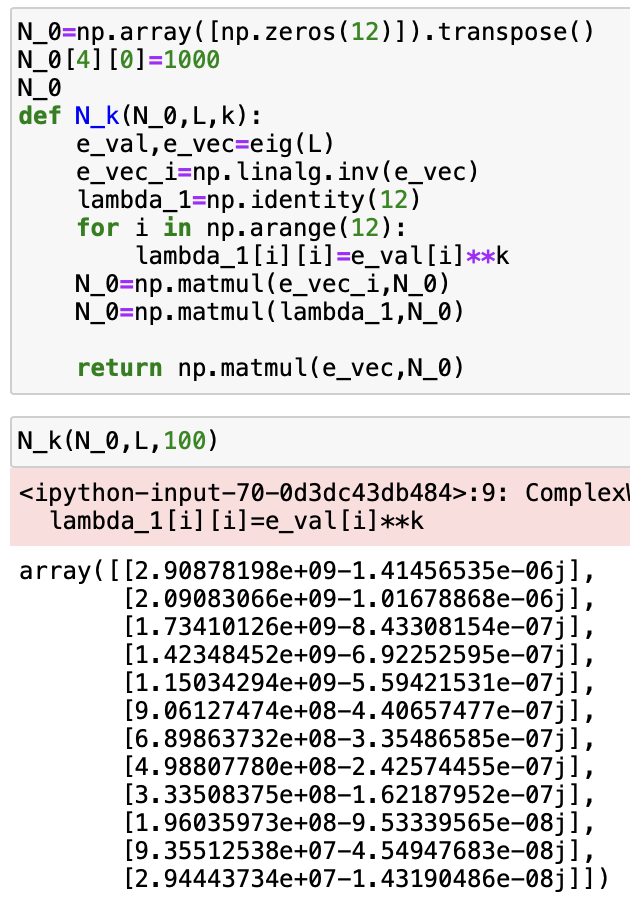
\includegraphics[scale=0.6]{Screenshot 2023-10-19 at 7.41.42 PM.png}
	\end{figure}
	\part What is the stable age distribution?
	\begin{figure}[h!]
		\centering
		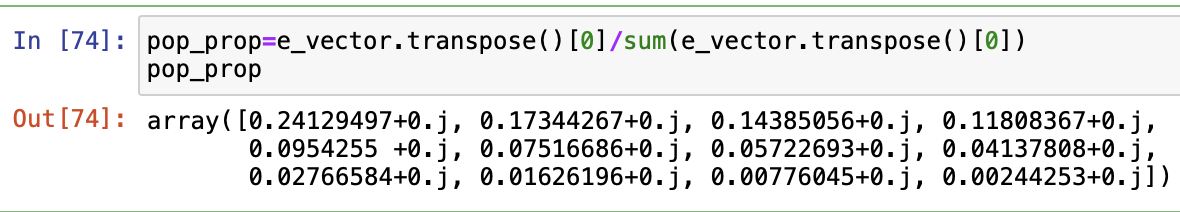
\includegraphics[scale=0.6]{Screenshot 2023-10-19 at 7.45.30 PM.png}
	\end{figure}
	\part New Zealand sheep farmers cannot live entirely on their income from wool, especially if they have to keep feeding ever more sheep. A desirable goal for management of a sheep herd (or any renewable resource) is to find a stable configuration from which one can harvest the {\it growth} at regular intervals, thereby producing income and returning the population to its previous configuration. A sustainable harvesting policy is a plan for harvesting on a regular schedule in such a way that the harvest is always the same and the state of the population after harvesting is always the same. \\
	
	Let $h_i$ be the fraction of the $i$-th age group that will be harvested at the end of each growth period and $H$ be the diagonal matrix whose entries are the $h_i$'s. For the previous parts, $N^{(k+1)}=LN^{(k)}$ but now if we consider the harvest after the growth, $N^{(k+1)}=LN^{(k)}-HLN^{(k)}=(I-H)LN^{(k)}$.
	\begin{enumerate}[(i)]
		\item We want a stable population, i.e. not changing at all. What eigenvalue corresponds to a stable population?\\
		An eigenvalue less than or equal to $1$ $1$ corresponds to a stable population
		\item What conditions are on $h_i$'s to have stable population?\\
		Choose $H$ s.t $\det((I-H)L-I)=0$, so $(I-H)L$ has an eigenvalue of $1$.
	\end{enumerate}
	\part A uniform harvesting policy is one in which the same fraction $h$ is harvested from each age group. Explain why this means $h=1-\frac{1}{\lambda_0}$ ($\lambda_0$ is the largest eigenvalue). 
	In the long term, the population will grow according to the dominating eigenvalue-eigenvector pair, so we want $\lambda_0\vec(v_0)-\lambda_0 H\vec(v_0)=\vec{v_0}$
\end{parts}
	
%----------------------------------------------------------------------------------------------   
\question  Supppose that $$L=\left[\begin{array}{rr}2&4\\0.3&0\end{array}\right]$$ is the Leslie matrix for a population with two age classes. It's convenient to always use the computer to compute things for us, but we don't always have computers. Without using the computer or technology, compute the following 
\begin{parts}
	\part Determine both eigenvalues.
	Let $f(x):=\det(L-xI)=(2-x)(0-x)-1.2\Rightarrow\lambda_0=1-\sqrt{2.2},\lambda_1=1+\sqrt{2.2}$
	\part Find the stable age distribution.
	$x_1=\left(\begin{array}{c}
		4 \\
		\sqrt{2.2}-1
	\end{array}\right)$
	$p=\left(\begin{array}{c}
		\frac{4}{3+\sqrt{2.2}} \\
		\frac{\sqrt{2.2}-1}{3+\sqrt{2.2}}
	\end{array}\right)$
\end{parts}
%----------------------------------------------------------------------------------------------
\question In this question we are going to create a Leslie matrix model for the US population. We will have to collect data of birth and death rates from the National Center for Health Statistics.\\

\indent You can download the most recent (2017) data on mortality rates from:
\url{https://ftp.cdc.gov/pub/Health_Statistics/NCHS/Publications/NVSR/68_07/}\\

\indent The different tables break the data down by race and by sex-at-birth. Table01 aggregates the data over the entire population. This is the table that we will use. The probability of dying data are all in column B.\\

\indent For birth rates we will use the data from 2017 published in Table 2 (Page 13) of the report:

\url{https://www.cdc.gov/nchs/data/nvsr/nvsr68/nvsr68_13-508.pdf}

\indent One wrinkle - birth rates are reported for women, but our population model includes all individuals (including non-women). Assume that a fraction $0.508$ of individuals are women (also based on CDC data). So multiply birth rates by $0.508$ to account for the fact that we must find the fraction of individuals in the age group who are women, and then find the fraction of births.\\

\indent Your first goal is to assemble a Leslie matrix using all of these data. For the birth rate data, which is aggregated over 5 years - e.g. 20-24 it is acceptable to assume that all ages in the group have the same birth rate - i.e. use the same birth rate for 20, 21, 22, 23 and 24 year olds. There is no need to write out or print the matrix - just use it to answer the questions.
\begin{parts}
	\part Why might it be inaccurate to assume that the same fraction of individuals in each age group are women? In other words why might different age groups have different fractions of women?\\
	One reason is that women on average live longer than men, so we'd expect to see a higher percentage of women in older populations. Other external factors such as a war could affect the proportion of each gender for a given age group.
	\part Use Python (or fab software) to calculate the largest eigenvalue of your matrix. Is it larger than 1, meaning that the population will increase over time?\\
	the largest eigenvalue is $0.9956059820629688$ which is less than $1$, so the population is decreasing.
	\part Find for yourself the most recent data on the distribution of ages of individuals in the US (cite the website or source that you used). Using your Leslie matrix model, predict how the populations will grow or decay over the next 100 years. Demonstrate your answer by making the following plots:\\ 
	\url{https://www.kff.org/other/state-indicator/distribution-by-age/?dataView=1&currentTimeframe=0&selectedRows=%7B%22wrapups%22:%7B%22united-states%22:%7B%7D%7D%7D&sortModel=%7B%22colId%22:%22Location%22,%22sort%22:%22asc%22%7D}
	\begin{enumerate}[(i)]
			\item The total population over time.
			\begin{figure}[H]
				\centering
				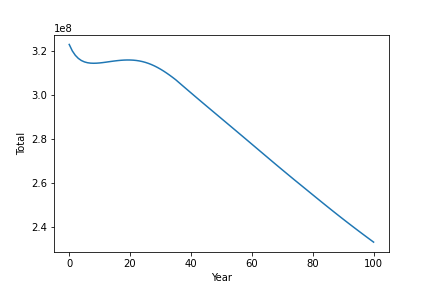
\includegraphics[scale=0.6]{Total vs Time.png}
			\end{figure}
			\item The number of people over the age of 65 as a fraction of the total population size.
			\begin{figure}[H]
				\centering
				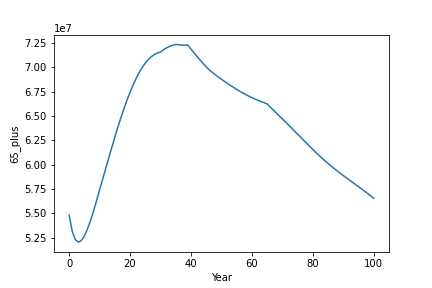
\includegraphics[scale=0.6]{65+ vs Time.png}
			\end{figure}
			\item The number of college age (i.e. 18-25) people as a function of the total population size.
			\begin{figure}[H]
				\centering
				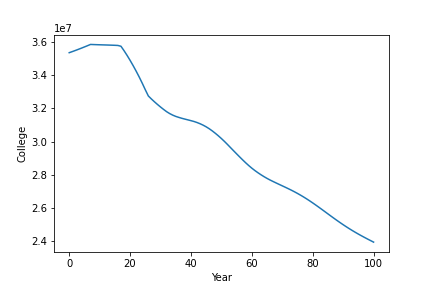
\includegraphics[scale=0.6]{College vs Time.png}
			\end{figure}
		\end{enumerate}
	\part What important effect did we miss when trying to predict demographic change in the US?\\
	Immigration and emmigration.
\end{parts}

%---------------------------------------------------------------------------------------------- 
%\question 
%\begin{parts}  
%	\part Create a model of a pair of dice analogous to the coin model where there is an equal probability for each of the 6 numbers on each die. Run the model 100 times and make a graph of the resulting distribution. (Do NOT google for this code. Just tweak the coin model.) Plot the results.
%	\part Create a second version where the dice are biased so that there is a $30\%$ greater chance of a six on each die. Plot the results.
%	\part Compare the two graphs and describe the results. 
%\end{parts}
%----------------------------------------------------------------------------------------------
\question Submit the code you used for any and all of the problems. (Print pdf the code) If we have any questions, we may ask you for the actual code file.\\
Used for data: \url{https://www.kff.org/other/state-indicator/distribution-by-age/?dataView=1&currentTimeframe=0&selectedRows=%7B%22wrapups%22:%7B%22united-states%22:%7B%7D%7D%7D&sortModel=%7B%22colId%22:%22Location%22,%22sort%22:%22asc%22%7D}\\
\begin{figure}[H]
\centering
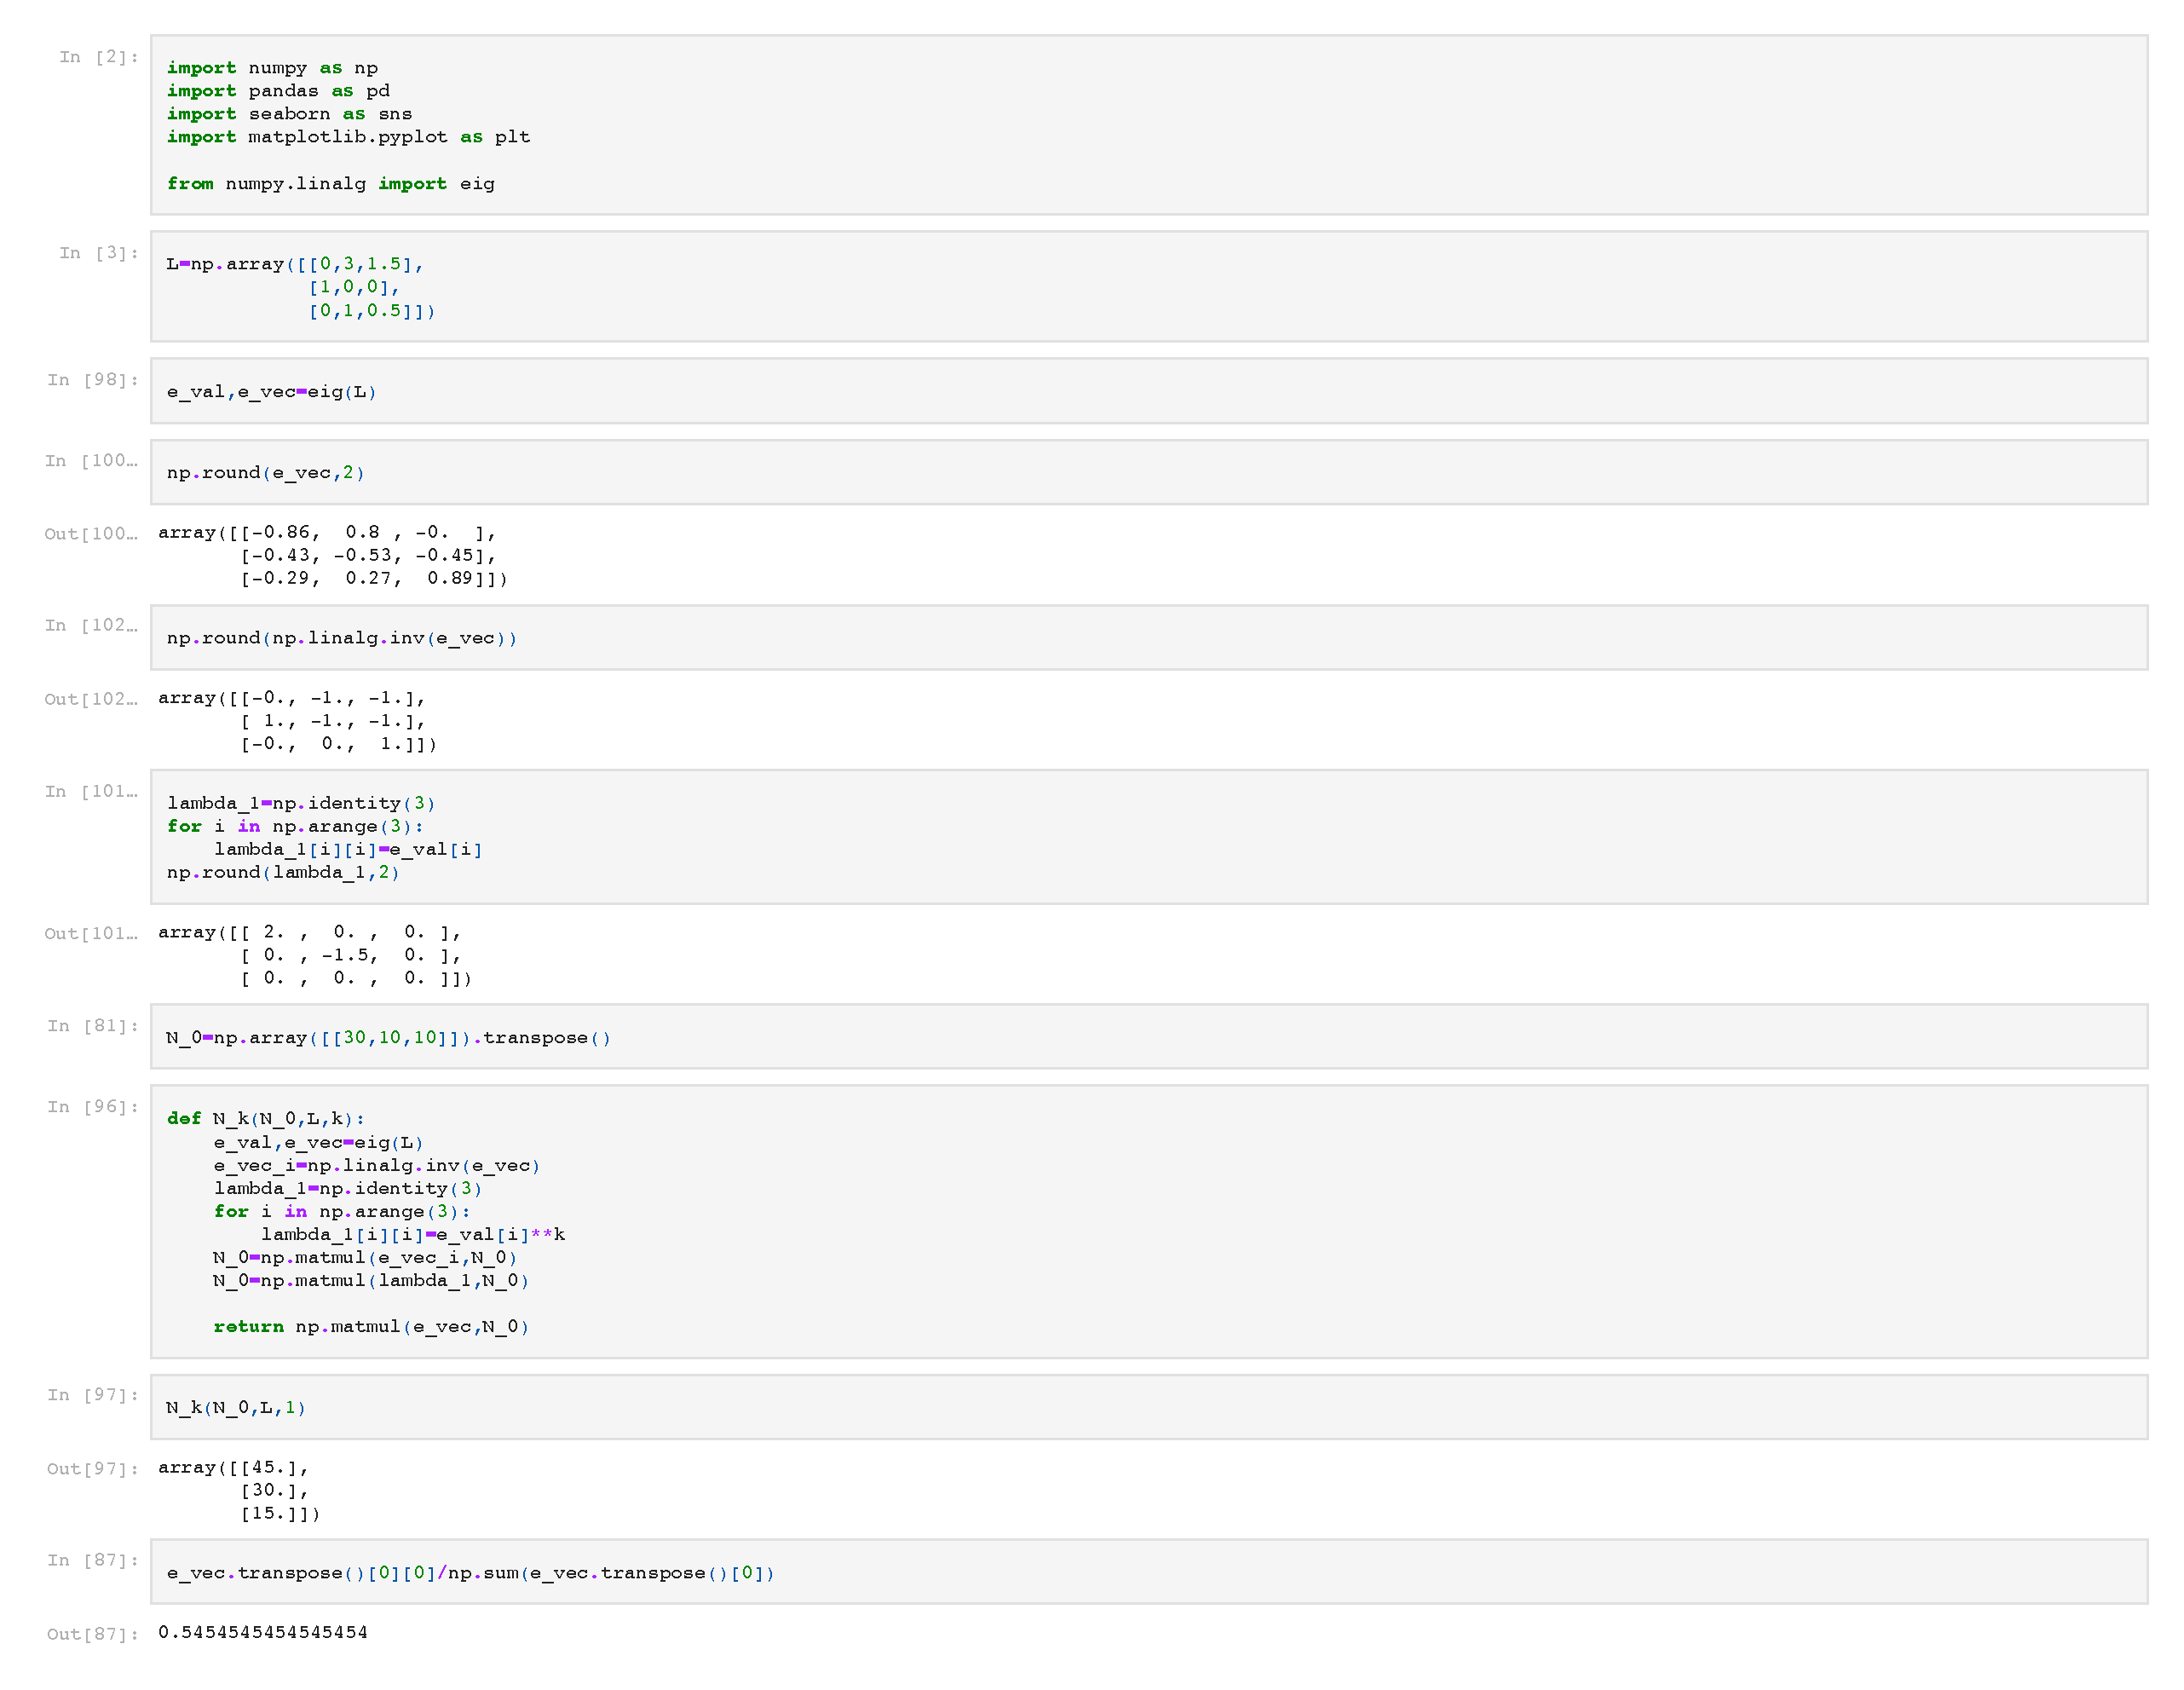
\includegraphics[scale=0.4]{Math_142_Homework_3_Q_1-Copy1.pdf}	
\end{figure}
\begin{figure}[H]
	\centering
	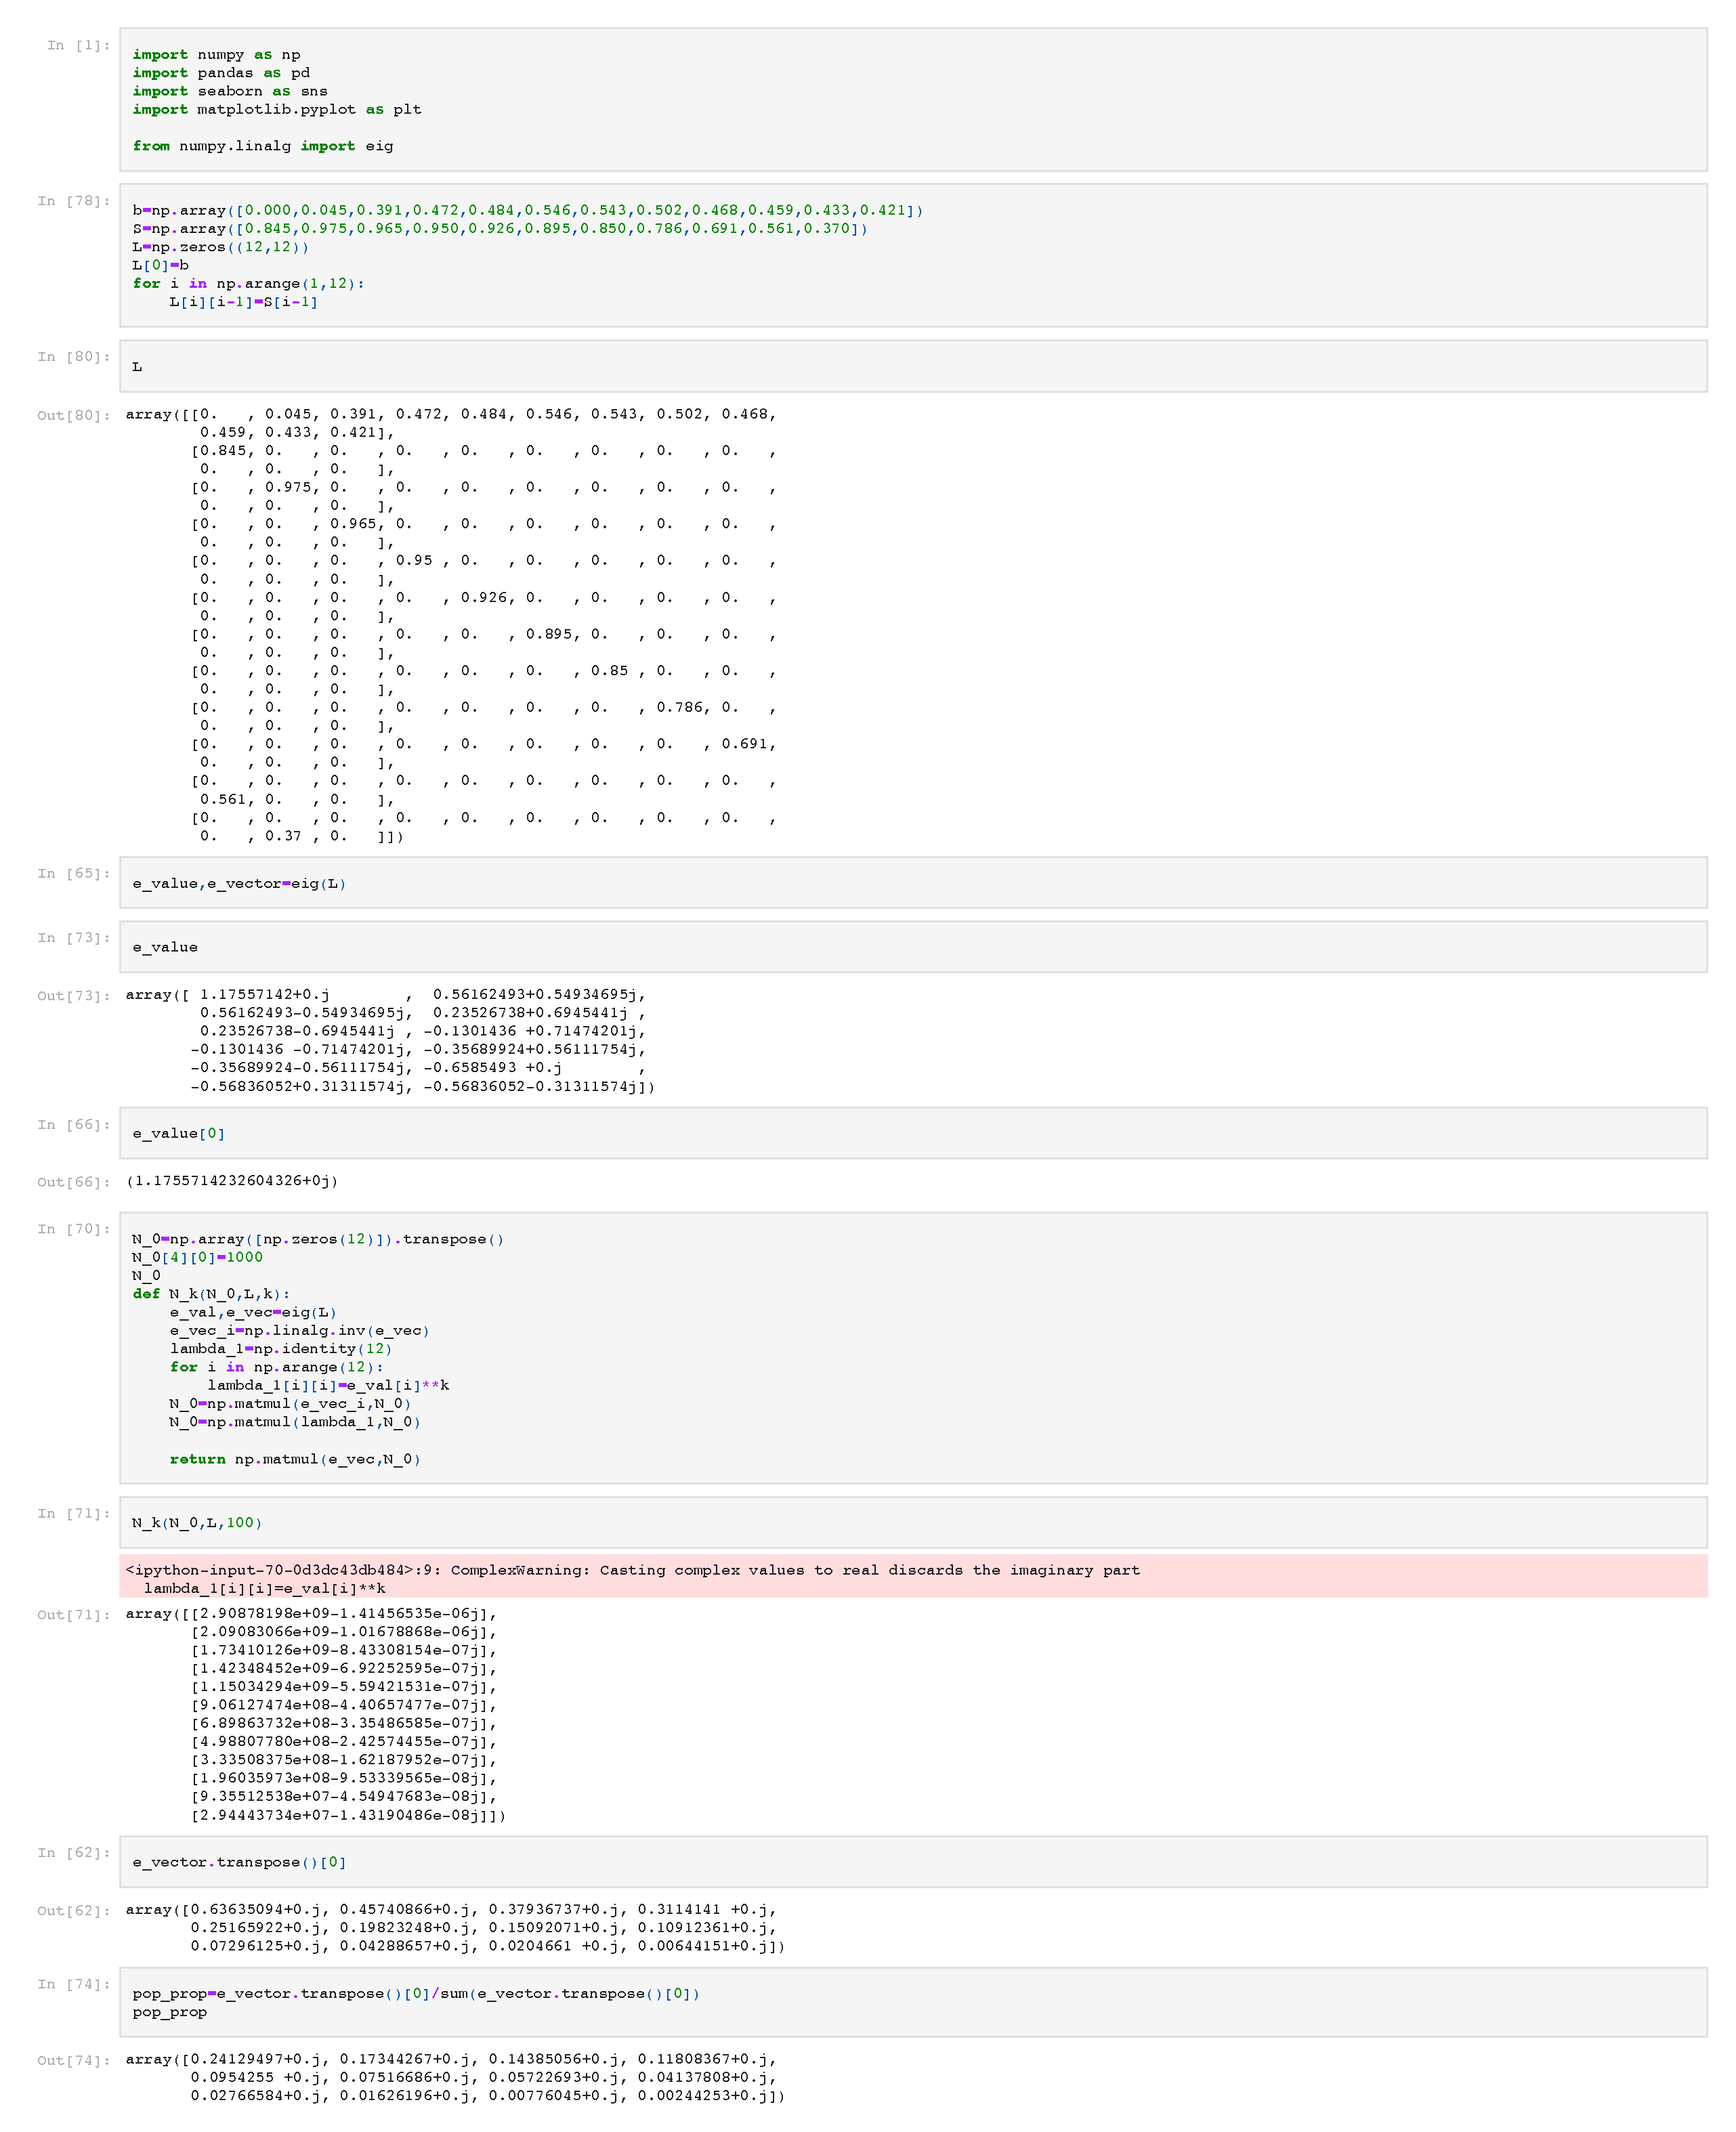
\includegraphics[scale=0.4]{Math_142_Homework_3_Q_2.pdf}	
\end{figure}
\begin{figure}[H]
	\centering
	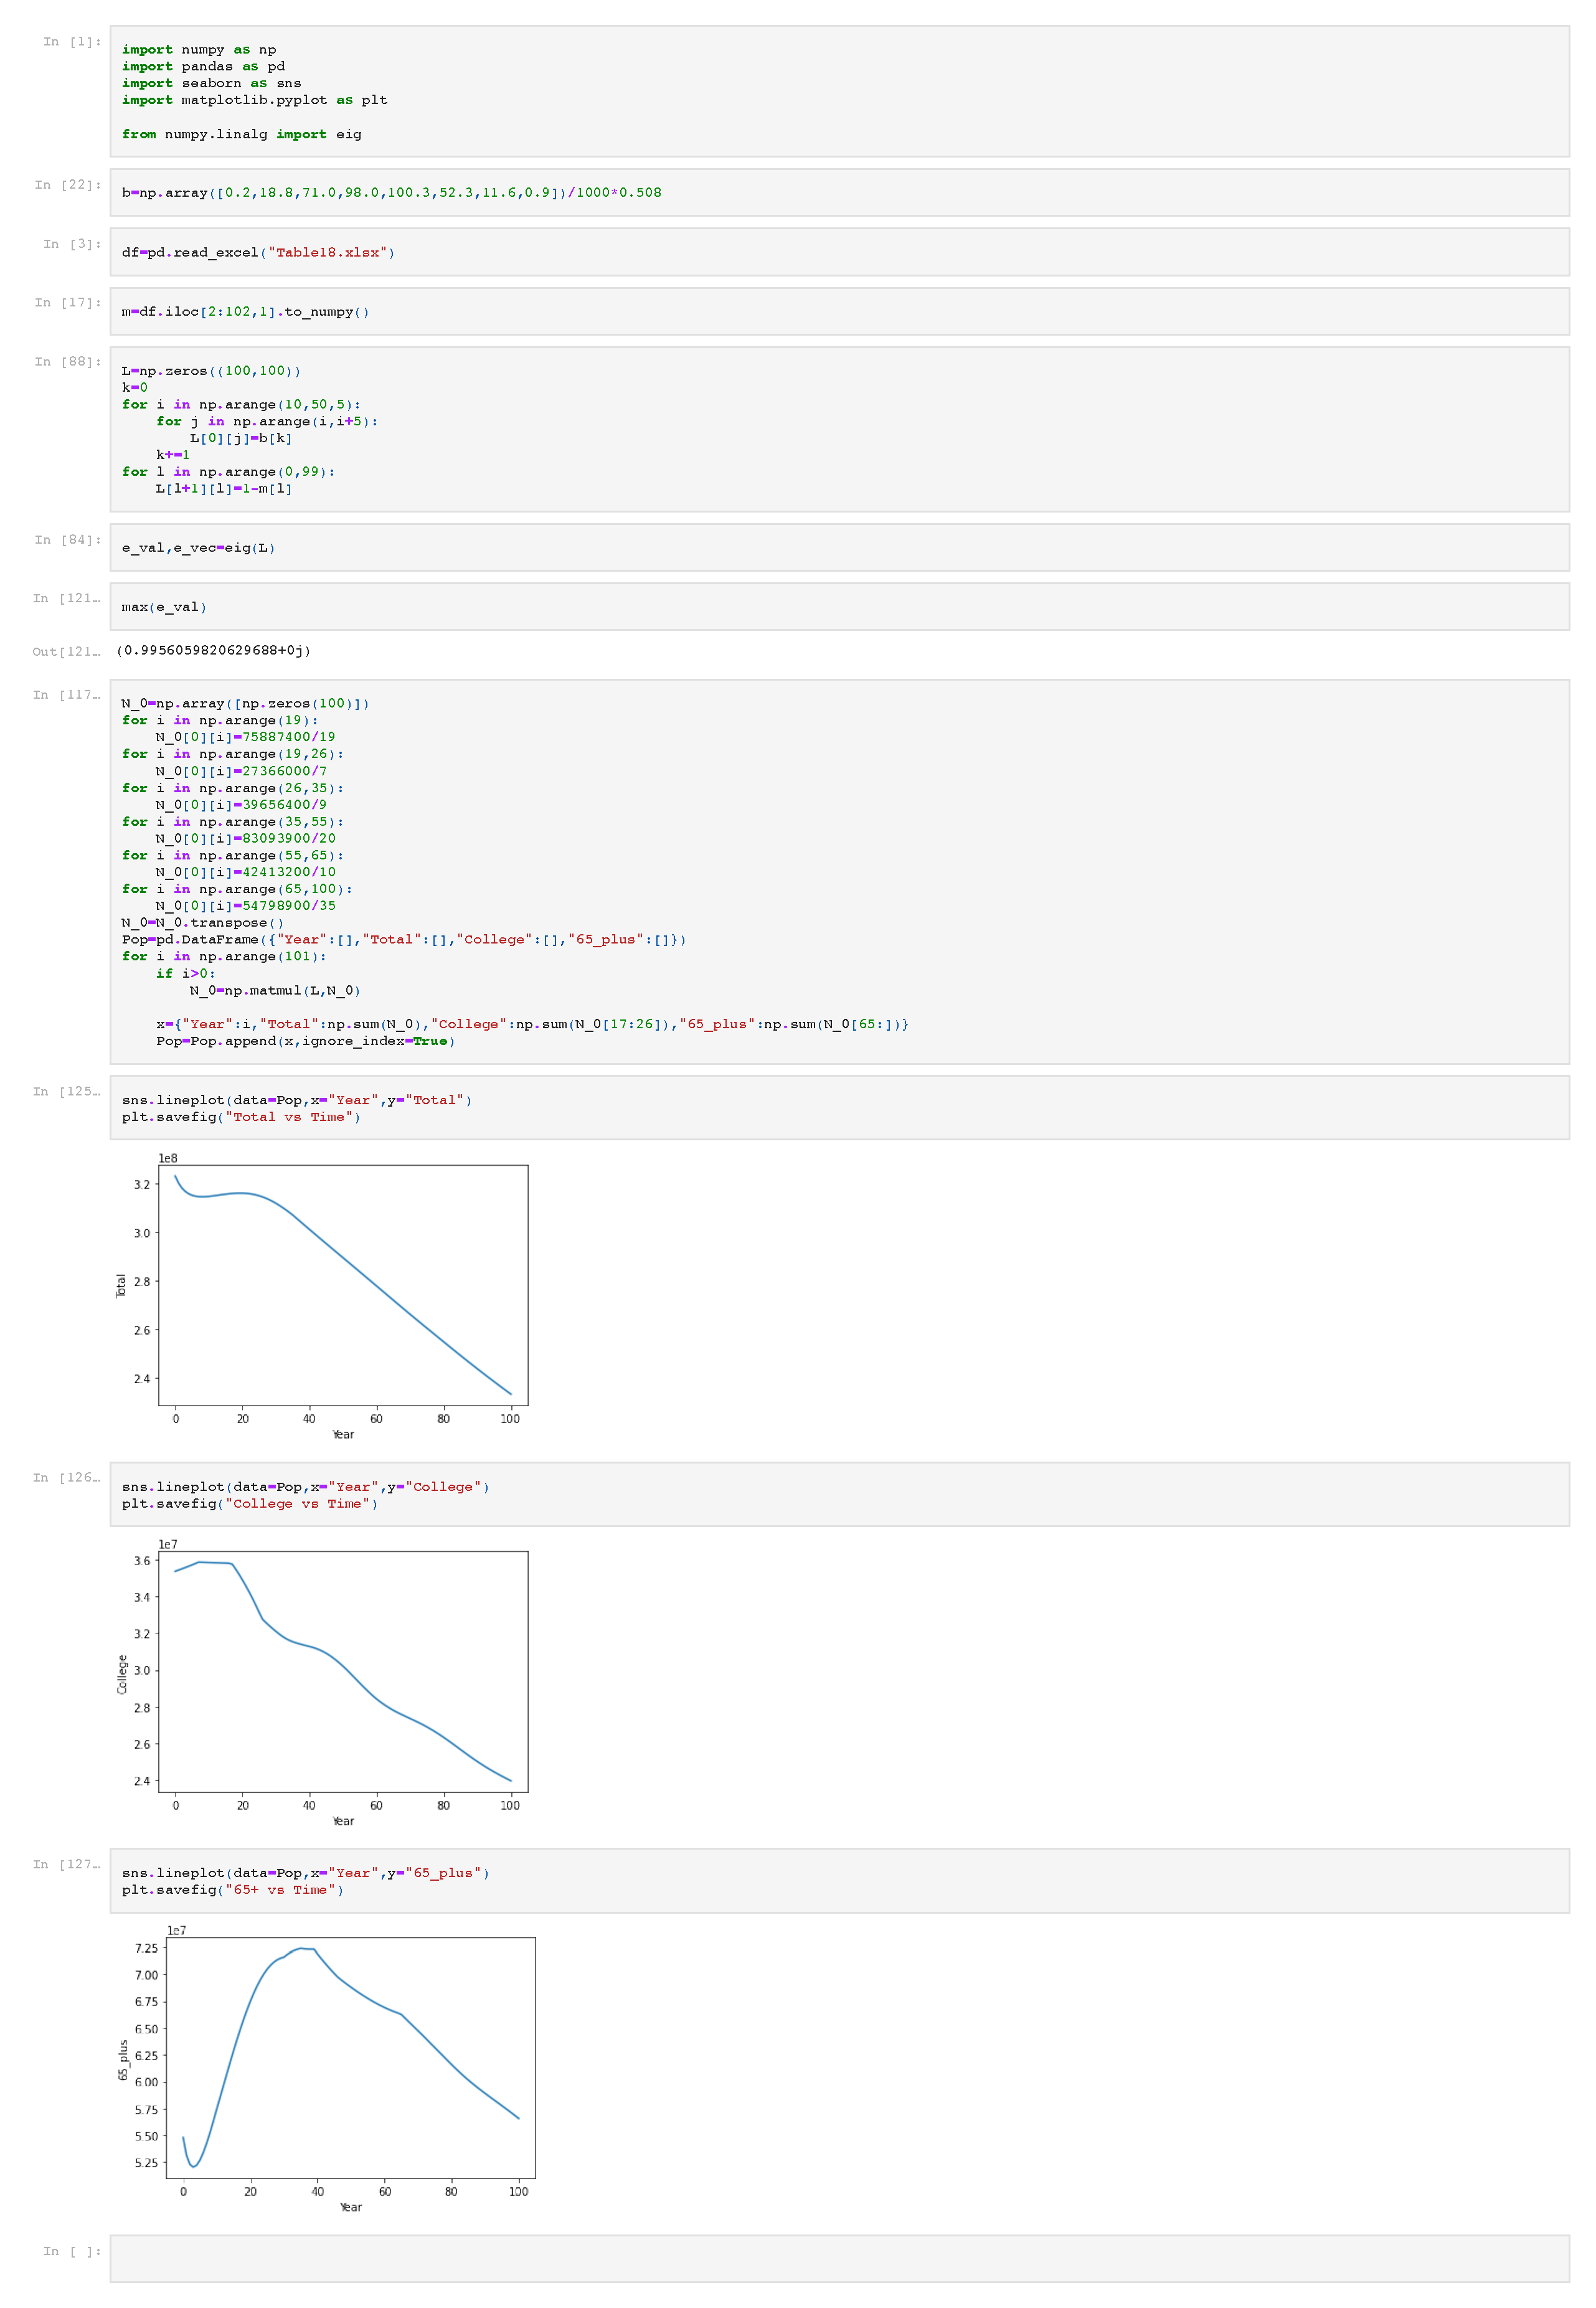
\includegraphics[scale=0.4]{Math_142_Homework_3_Q_4.pdf}	
\end{figure}
%----------------------------------------------------------------------------------------------

\end{questions}
%\end{multicols*}
\end{document}